\section{Introduction}\label{intro}

When we consider running the software correlator on a grid then the problem of communication between grid clusters arises. It will be a good idea to summerize the process of grid computing to get a broader idea. As stated in \cite{dj14} (for detailed explanation please see reference \cite{dj14}):

\begin{figure}[h!]
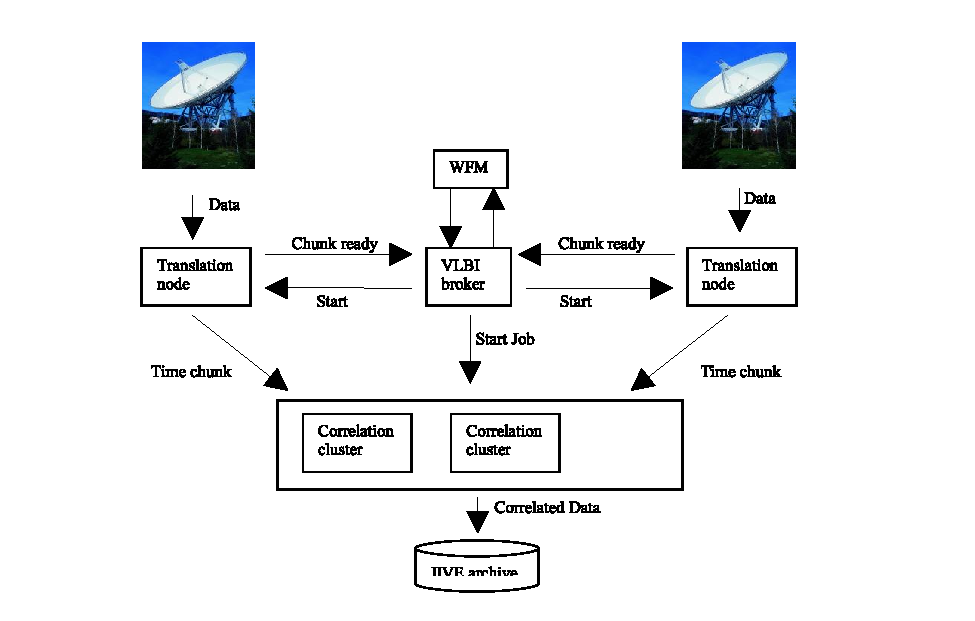
\includegraphics[width=15cm, angle=0]{figures/grid.eps}
\caption{Distribution at grid level.}
\end{figure} 

\begin{itemize}
\item The The Work Flow Manager (WFM) starts the correlation process. The user specifies a VEX file and the WFM converts it to a CCF file. WFM notifies VLBI Broker about the new experiment, which is responsible for managing the further process.
\item The VLBI broker starts the translation nodes, which open a connection to a telescope. 
\item The translation nodes send messages back to the broker when time chunks are available. It is the task of the translation node to buffer the data and to chop the incoming data stream into chunks.  
\item When a time chunk is available for all telescopes, the VLBI broker sends a start message to the translation and the correlation nodes. The translation nodes send the data to the correlation clusters which do the processing.
\item After the correlation of the chunk the output of all time chunks is transferred to a central location from which JIVE can retrieve the data using grid FTP
\end{itemize}

